\documentclass[12pt]{article}
\title{Convolutional Neural Network}
\author{Le Chi Thanh - M23.ICT.011}
\date{\today}

\usepackage{verbatim}
\usepackage{listings}
\usepackage{graphicx}
\usepackage{caption}
\usepackage{biblatex}
\usepackage{amsmath}
\addbibresource{citation-336805909.bib}

\begin{document}
\maketitle

In this report, we present the implementation of VGG19, a convolutional neural network (CNN) architecture, for image classification.

\section{Methodology}

\subsection{Dataset}

For this project, we utilized a dataset comprising images of celebrities. The dataset is organized into directories, each containing images of a specific celebrity. The celebrities included in the dataset are Maria Sharapova, Lionel Messi, Cristiano Ronaldo, Shah Rukh Khan, and Virat Kohli. This dataset serves as the basis for training and evaluating our image classification model.

\subsection{Data Preprocessing}

\begin{verbatim}
train_datagen = ImageDataGenerator(
    rescale=1./255,            # Normalize pixel values to [0, 1]
    shear_range=0.2,           # Randomly shearing transformations
    zoom_range=0.2,            # Randomly zoom into images
    horizontal_flip=True,      # Randomly flip images horizontally
    validation_split=0.2       # train/validation=80/20
)

train_generator = train_datagen.flow_from_directory(
    train_data_dir,
    target_size=(224, 224),    # Resize all images to 224x224
    batch_size=32,             # Number of images per batch
    class_mode='categorical',  # Use categorical labels
    subset='training',         # Use the training subset
    shuffle=True
)

validation_generator = train_datagen.flow_from_directory(
    train_data_dir,
    target_size=(224, 224),    # Resize all images to 224x224
    batch_size=16,             # Number of images per batch
    class_mode='categorical',  # Use categorical labels
    subset='validation',       # Use the validation subset
    shuffle=True
)
\end{verbatim}

Before feeding the images into the model, we performed data preprocessing to ensure consistency and enhance model performance. The process include:

\begin{itemize}
  \item \textbf{Resizing}: Resizing ensures that all images are brought to a uniform size as convolutional neural networks (CNNs) like VGG19 require fixed-size input. In this case, all images are resized to a common size of 224x224 pixels.
  \item \textbf{Normalization}: Pixel values in images range from 0 to 255 for each color channel (red, green, and blue). In this implementation, pixel values are divided by 255 to rescale them to the range [0, 1].
  \item \textbf{Augmentation}: Data augmentation is a technique used to artificially increase the diversity of the training dataset by applying random trans-formations to the images. Augmentation techniques in this report include:
  \begin{itemize}
    \item \textbf{Shearing}: Applying a shear transformation to the images, which slants the shape of the objects.
    \item \textbf{Zooming}: Randomly zooming into or out of the images.
    \item \textbf{Horizontal flipping}: Flipping images horizontally.
  \end{itemize}
  \item \textbf{Train and Test(Validation) dataset split}: In this experiement, 80\% of the data is used for training (subset='training'), while the remaining 20\% is set aside for validation (subset='validation'). 
  \item \textbf{Classìication Mode}: For image classification tasks, labels are represented as categorical variables, where each image belongs to one of multiple classes.
  
\end{itemize}

\subsection{Discussion on Convolutional Neural Network}

    \begin{figure}[h]
        \centering
        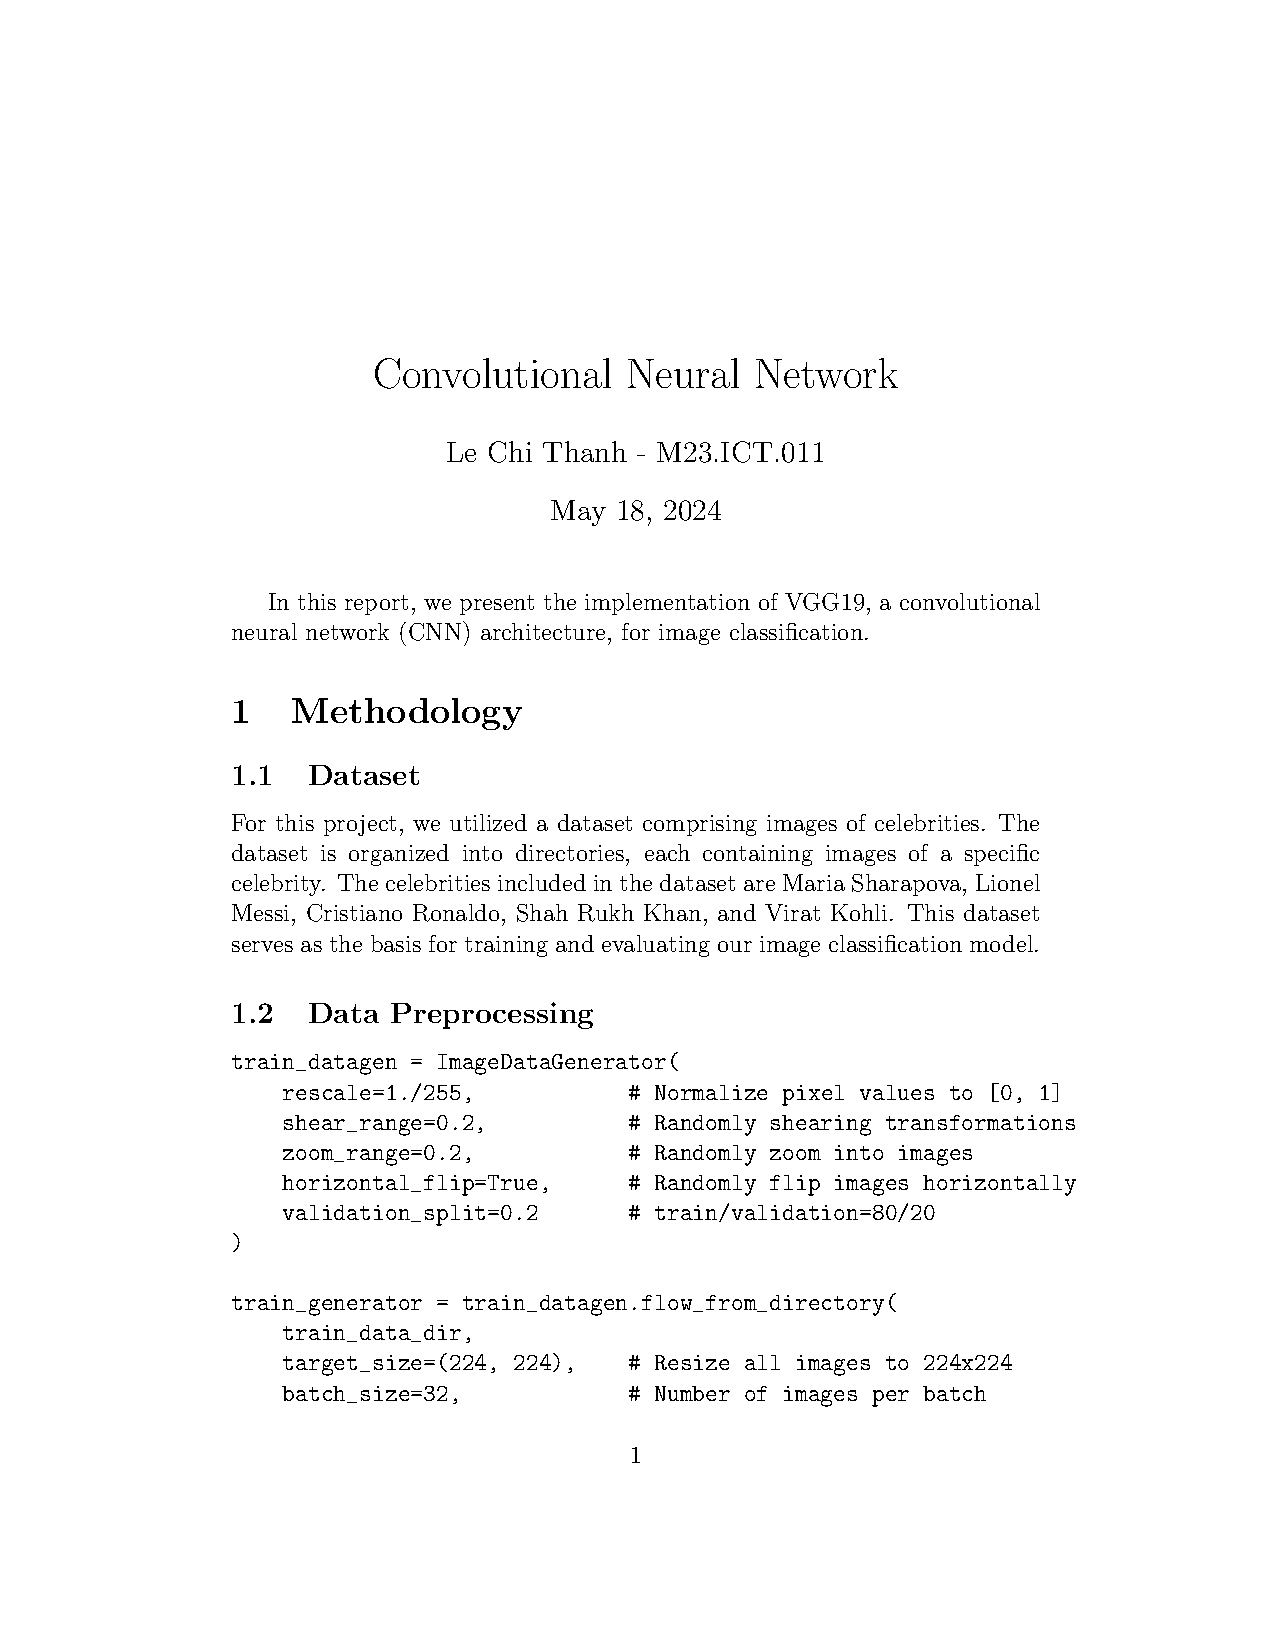
\includegraphics[width=0.8\linewidth]{CNN.jpg}
        \caption{Convolutional Neural Network architecture. Source: \cite{article}}
        \label{fig:enter-label}
    \end{figure}
    
To further understanding and later explaning the VGG19 model architecture. We will discuss some basic concept on Convolution Neural Network (CNN) here. The basic architecture of CNN is designed to extract meaningful features from complex visual data, these meaning ful features would be transform to neurons' weights in the neural network with hidden layers. This is achieved through the use of specialized layers within the network architecture, it comprises three fundamental types:

    \begin{enumerate}
        \item \textbf{Convolutional Layers}: Compute a dot product between the \textbf{filter/kernel value} and the \textbf{image pixel values}. The matrix formed by sliding the filter over the image is called the \textbf{Convolved Feature, Activation Map, or Feature Map}.

        The behavior of the convolutional layer is governed by the following parameters:

        \begin{itemize}
            \item \textbf{Kernel size (or filter size):} It determines the size of the kernel window/filter matrice. In VGG19 we use a kernel with size (3,3) featuring a 3x3 matrice (or tensors).
            \item \textbf{Stride:} The stride parameter determines the number of pixels the kernel window will move during each step of convolution. In VGG19 we set this parameter to 1 to avoid missing features from image.
            \item \textbf{Padding:}  Padding refers to the technique of adding zeros to the border of an image. By applying padding, the kernel can fully filter every position of an input image, ensuring that even the edges are properly processed. Later on in VGG19, we are going to have padding='same' ensures that the output has the same width and height as the original input by padding zeros to the input images.
            \item \textbf{Number of filters /Depth:} While each filter is actually a 3x3 matrices with different weights, the number of filters in a convolutional layer determines the number of patterns or features that the layer will seek to identify. In other words, it governs the number of distinct characteristics or elements that the convolutional layer will focus on detecting. Later on with VGG19, we let Tensorlow/Keras to automatically generate the filter matrices.
        \end{itemize}

        \textbf{E.g:} Let's take into example and solve an convolutional layer in math language. In the example we got one input(224,224,3) and a convolutional layer (64,(3,3)):
        \begin{enumerate}
            \item \textit{Input Dimensions:} Image 224x224x3
            \item \textbf{Convolution Operation:} Numeber of filters (depth) = 64; Kernel size: (3,3); Stride: 1; Padding: 1 (Same)
            \item \textbf{Output Caculation:} We apply the formula to caculate output height/width - in this case they are same:
            \[\text{O-H/W} = \left( \frac{\text{I-H/W} - \text{Kernel Size} + 2 \times \text{Padding}}{\text{Stride}} \right) + 1\]
            For the convolutional layer:
            \[\text{O-H/W} = \left( \frac{224 - 3 + 2 \times 1}{1} \right) + 1  = 224\]
            Thus, the output feature map is 224x224 for each of the 64 filters.
            \item \textbf{Summary:}
            \begin{itemize}
                \item Input dimension: 224x224x3 (RGB Image)
                \item Output Dimension after Convolutional Layer: 224x224x64 (Same Image size, 64 features extracted).
            \end{itemize}
        \end{enumerate}

        When the input has more than one channel (e.g. an RGB image), the filter should have a matching number of channels. To calculate one output cell, we perform convolution on each matching channel, then add the result together (Figure 3).
        
        \begin{figure}[h]
        \centering
        \includegraphics[width=0.5\linewidth]{ConvoLayer.png}
        \caption{Convolutional Process}
        \label{fig:enter-label}
        \end{figure}

        \begin{figure}[h]
        \centering
        \includegraphics[width=0.8\linewidth]{RGBConvoLayer.png}
        \caption{Convolutional on RGB Image}
        \end{figure}

        After the convolution operation, the resulting feature map may contain negative values as well as positive values. Applying ReLU to the feature map:

        \[\text{Output} = \text{ReLU}(\text{Feature Map})\]

        \begin{itemize}
            \item ReLU (Rectified Linear Unit) is defined as:
            \[\text{ReLU}(x) = \max(0, x)\]   
            \item It sets all negative values in the feature map to zero and preserves positive values unchanged.
            \item This operation enhances the non-linear properties of the decision function and of the overall network without affecting the receptive fields of the convolution process.
        \end{itemize}

        \item \textbf{Pooling Layers}: also referred to as downsampling, serve to \textit{reduce the dimensionality} of the input. Similar to convolutional layers, pooling operations involve traversing a filter across the input. However, unlike convolutional layers, the pooling filter does not possess weights. Instead, the filter applies an aggregation function to the values within its receptive field, generating the output array. Two primary types of pooling are commonly employed:
        \begin{itemize}
            \item \textbf{Max Pooling:} Selects the pixel with the maximum value to send to the output array.
            \item \textbf{Average pooling:} It calculates the average value within the receptive field to send to the output array.
        \end{itemize}

        In the VGG19 Model, we mostly use MaxPooling with a filter/pooling window of 2x2 and a stride of (2, 2) - means the pooling window moves 2 units at a time along both the height 
        and width dimensions of the input.

        \begin{figure}[h]
        \centering
        \includegraphics[width=0.5\linewidth]{MaxPooling.png}
        \caption{Max Pooling}
        \end{figure}
        
        \item \textbf{Fully-Connected Layers}: The Fully Connected Layer or dense layer aims to provide global connectivity between all neurons in the layer. Unlike convolutional and pooling layers, which operate on local spatial regions, the fully connected layer connects every neuron to every neuron in the previous and subsequent layers. 

        The fully connected layer typically appears at the end of the CNN architecture, firstly beging with the \textbf{flatten layers and dense layers}, which take the flattened feature maps from the preceding convolutional and pooling layers as input. 

        \textbf{E.g:} We take an example of a flatten and dense process:
        
        \textit{\textbf{Fully connected layers}}
        \\ x = Flatten(name='flatten')(x)
        \\ x = Dense(4096, activation='relu', name='fc1')(x)
        \\\textit{\textbf{Output layer}}
        \\outputs = Dense(5, activation='softmax', name='predictions')(x)
        
        \begin{enumerate}
            \item Flatten Layer: 7x7x512 = 25088 weights (vector shape: 25088x1)
            \item First Dense Layer: Input:25088; Weights(25088,4096); Bias: 4096; Output:4096 (vector shape: 4096x1)
            \item First Dense Caculation: While ReLU is the activation function, the output weight z of the dense layer is computed as:
            \[\text{z} = \text{ReLU(Wx+Bias)}\]
            \item Second Dense Layer (Output Layer): Input:4096; Weights(4096,5); Bias: 5; Output: 5 (vector shape: 5x1). 5 is the number of desired class/label in this example.
            \item Second Dense Layer Caculation: While Softmax is the activation, the output weights z of the dense layer is computed as:
            \[\text{softmax}(z_i) = \frac{e^{z_i}}{\sum_{j=1}^{n} e^{z_j}}\]
            where \( z_i \) is the \( i \)-th element of the input vector \( z \), and \( n \) is the number of classes.
            \item The softmax function ensures that the output values are in the range (0,1) and that they sum to 1. This makes the output interpretable as probabilities, which is especially useful for multi-class classification tasks.
        \end{enumerate}

        These dense layers effectively reduces the spatial dimensions while transforming the data into a format suitable for fully connected layers, allowing the neural network to learn high-level representations.
    \end{enumerate}
	
\subsection{Model Architecture (VGG19)}

The VGG19 model architecture is a deep convolutional neural network (CNN) that was proposed by Karen Simonyan and Andrew Zisserman in 2014. It belongs to the VGG (Visual Geometry Group) family of models developed at the University of Oxford, and it is named after the "Visual Geometry Group" research group. VGG19 is an extension of the original VGG16 model, with the number "19" representing the total number of layers (including convolutional and fully connected layers) in the network. We explain the architecture in detail:

\begin{itemize}
  \item Input: (224, 224, 3) images.
  \item Convolutional Layers:  16 Convolutional layers in total, organized into five blocks with increasing filter counts (64, 128, 256, 512).
  \item Pooling Layers: 5 MaxPooling layers, each following a set of Convolution layers.
  \item Fully Connected Layers: 2 dense layers with 4096 node/neurons each.
  \item Output Layer: 1 dense layer with 5 node/neurons and softmax activation for classification.
\end{itemize}

The model is compiled into a Keras Model object, which can then be trained on a dataset for tasks such as image classification. The softmax output layer indicates that this specific implementation is designed for a 5-class classification problem.

\subsection{Training Setup}

Explain batchsize, epoch, validation step

Batching: In deep learning, it's common to process data in batches rather than all at once. Batching helps improve memory efficiency and speeds up the training process. The batch\_size parameter determines the number of images processed in each batch during training.

\section{Implementation}

\section{Result}

\section{Discussion}

\subsection{Analysis the results}

\subsection{Impact of training dataset qualitys}


% Print bibliography
\printbibliography

\end{document}
